\documentclass{beamer}
\usetheme[numbering=progressbar]{focus}
\usepackage{tikz}
\usetikzlibrary{positioning}
\usetikzlibrary{shapes,arrows}
\usepackage{transparent}
\usepackage{fancyvrb}
\usepackage{listings}
\definecolor{main}{RGB}{47, 161, 219}
%\definecolor{textcolor}{RGB}{128, 128, 128}
\definecolor{background}{RGB}{240, 247, 255}
\definecolor{textcolor}{RGB}{85, 87, 83}
\title{Snake Oil Crypto:}
\subtitle{How I stopped to worry and started to love crypto}
\author{Jean-Louis Huynen}
\titlegraphic{
\includegraphics[scale=0.20]{../../logos/d4-logo.pdf}}
\institute{Team CIRCL \\ \url{https://www.d4-project.org/}}
\date{2019/11/27}

\begin{document}
    \begin{frame}
        \maketitle
    \end{frame}

\begin{frame}
        \frametitle{Outline}

        \begin{itemize}
          \item Cryptography 101,
          \item Cryptography and Network captures,
          \item D4 passiveSSL Collection,
          \item Leveraging OpenPGP metedata,
          \item Checking for weak crypto.
        \end{itemize}

\end{frame}

\begin{frame}
  \begin{center}
    {\bf Cryptography 101}
  \end{center}
\end{frame}


\begin{frame}
  \frametitle{Cryptography Concepts}
        \begin{itemize}
          \item {\bf Plaintext} P: Text in clear,
          \item {\bf Encryption} E: Process of disguising the plaintext to hide its content,
          \item {\bf Ciphertext} C: Result of the Encryption process,
          \item {\bf Decryption} D: Process of reverting encryption, transforming C
            into P,
          \item {\bf Encryption Key} EK: Key to encrypt P into C,
          \item {\bf Decryption Key} DK: Key to decrypt C into P,
          \item {\bf Cryptanalysis}: Analysis of C to recover P without knowing K.
        \end{itemize}

\end{frame}

\begin{frame}
        \frametitle{Cryptography Services}

        \begin{itemize}
          \item {\bf Confidentiality }: Ensure the secrecy of the message except for
            the {\bf intended } recipient,
          \item {\bf Authentication }: Proving a party's identity,
          \item {\bf Integrity }: Verifying that data transmitted were not altered,
          \item {\bf Non-repudiation }: Proving that the sender sent a given message.
        \end{itemize}

\end{frame}

\begin{frame}
        \frametitle{Type of Encryption Applications}

        \begin{itemize}
          \item {\bf In-transit encryption}: protects data while it is
            transferred from one machine to another,
          \item {\bf At-rest encryption}: protects data stored on one machine.
          %\item {\bf Perfect Forward Secrecy}
        \end{itemize}

\end{frame}

\begin{frame}
        \frametitle{Kerckhoffs's Principle}

        \begin{quote}
          It [cipher] should not require secrecy, and it should not be a problem if it falls into enemy hands.
        \end{quote}

        \vspace{10 mm}

        { \bf There is no security in obscurity.}

\end{frame}


\begin{frame}[allowframebreaks]
        \frametitle{Attackers model}
        {\bf Black Box} - Attackers may only see inputs / outputs:
        \begin{itemize}
          \item {\bf Ciphertext-Only Attackers (COA) :} see only the ciphertext,
          \item {\bf Known-Plaintext Attackers (KPA):} see ciphertext and plaintext,
          \item {\bf Chosen-Plaintext Attacker (CPA):} encrypt plaintext, and
            see ciphertext, 
          \item {\bf Chosen-Ciphertext Attakers (CCA):} encrypt plaintext,
            decrypt ciphertext.
        \end{itemize}

        \framebreak

        {\bf Grey Box} - Attackers see cipher's implementation:
        \begin{itemize}
          \item {\bf Side-Channel Attacks:} study the behavior of the
            implementation, eg. {\bf timing attacks }\footnote{\url{https://cryptojedi.org/peter/data/croatia-20160610.pdf}}:
            \begin{itemize}

              \item Osvik, Shamir, Tromer~\cite{aes2006}: Recover AES-256 secret
                key of Linux’s dmcrypt in just 65 ms
              \item AlFardan, Paterson~\cite{lucky13}: “Lucky13” recovers plaintext of CBC-mode encryption in pretty much all TLS implementations
              \item Yarom, Falkner~\cite{gpg2014}: Attack against RSA-2048 in GnuPG 1.4.13: “On average, the attack is able to recover 96.7\% of the bits of the secret key by observing a single signature or decryption round.”
              \item Benger, van de Pol, Smart, Yarom~\cite{openssl2014}: “reasonable level of success in recovering the secret key” for OpenSSL ECDSA using secp256k1 “with as little as 200 signatures”

            \end{itemize}

        \framebreak
        Most recent timing attack: {\bf TPM-fail }~\cite{244048}

        \vspace{10 mm}

            \begin{figure}[h!]
              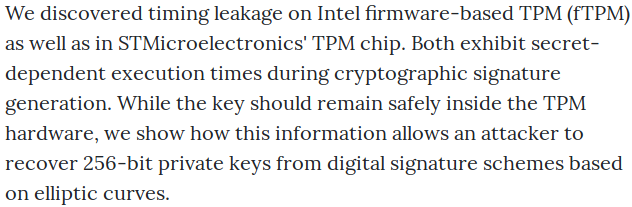
\includegraphics[width=250px]{./tpmfail.png}
            \end{figure}

        \framebreak

          \item {\bf Invasive Attacks:} 

            \begin{itemize}
              \item injecting faults~\cite{Matsuda2018},

                \vspace{10 mm}

                \begin{figure}[h!]
                  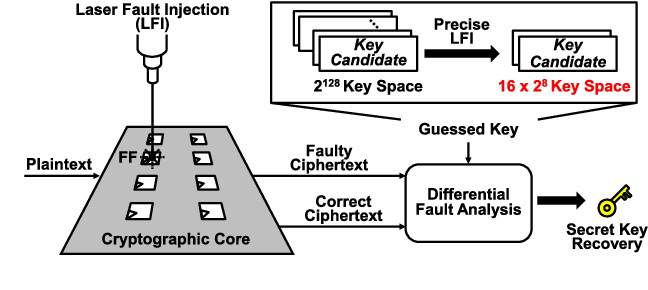
\includegraphics[width=250px]{./faultInjection.png}
                \end{figure}

        \framebreak

              \item decapping chips~\footnote{~\url{https://siliconpr0n.org/wiki/doku.php?id=decap:start}}, reverse engineering~\footnote{~\url{http://siliconzoo.org}}~\footnote{~\url{http://degate.org}}, etc.

           \end{itemize}
 
        \end{itemize}

                \begin{figure}[h!]
                  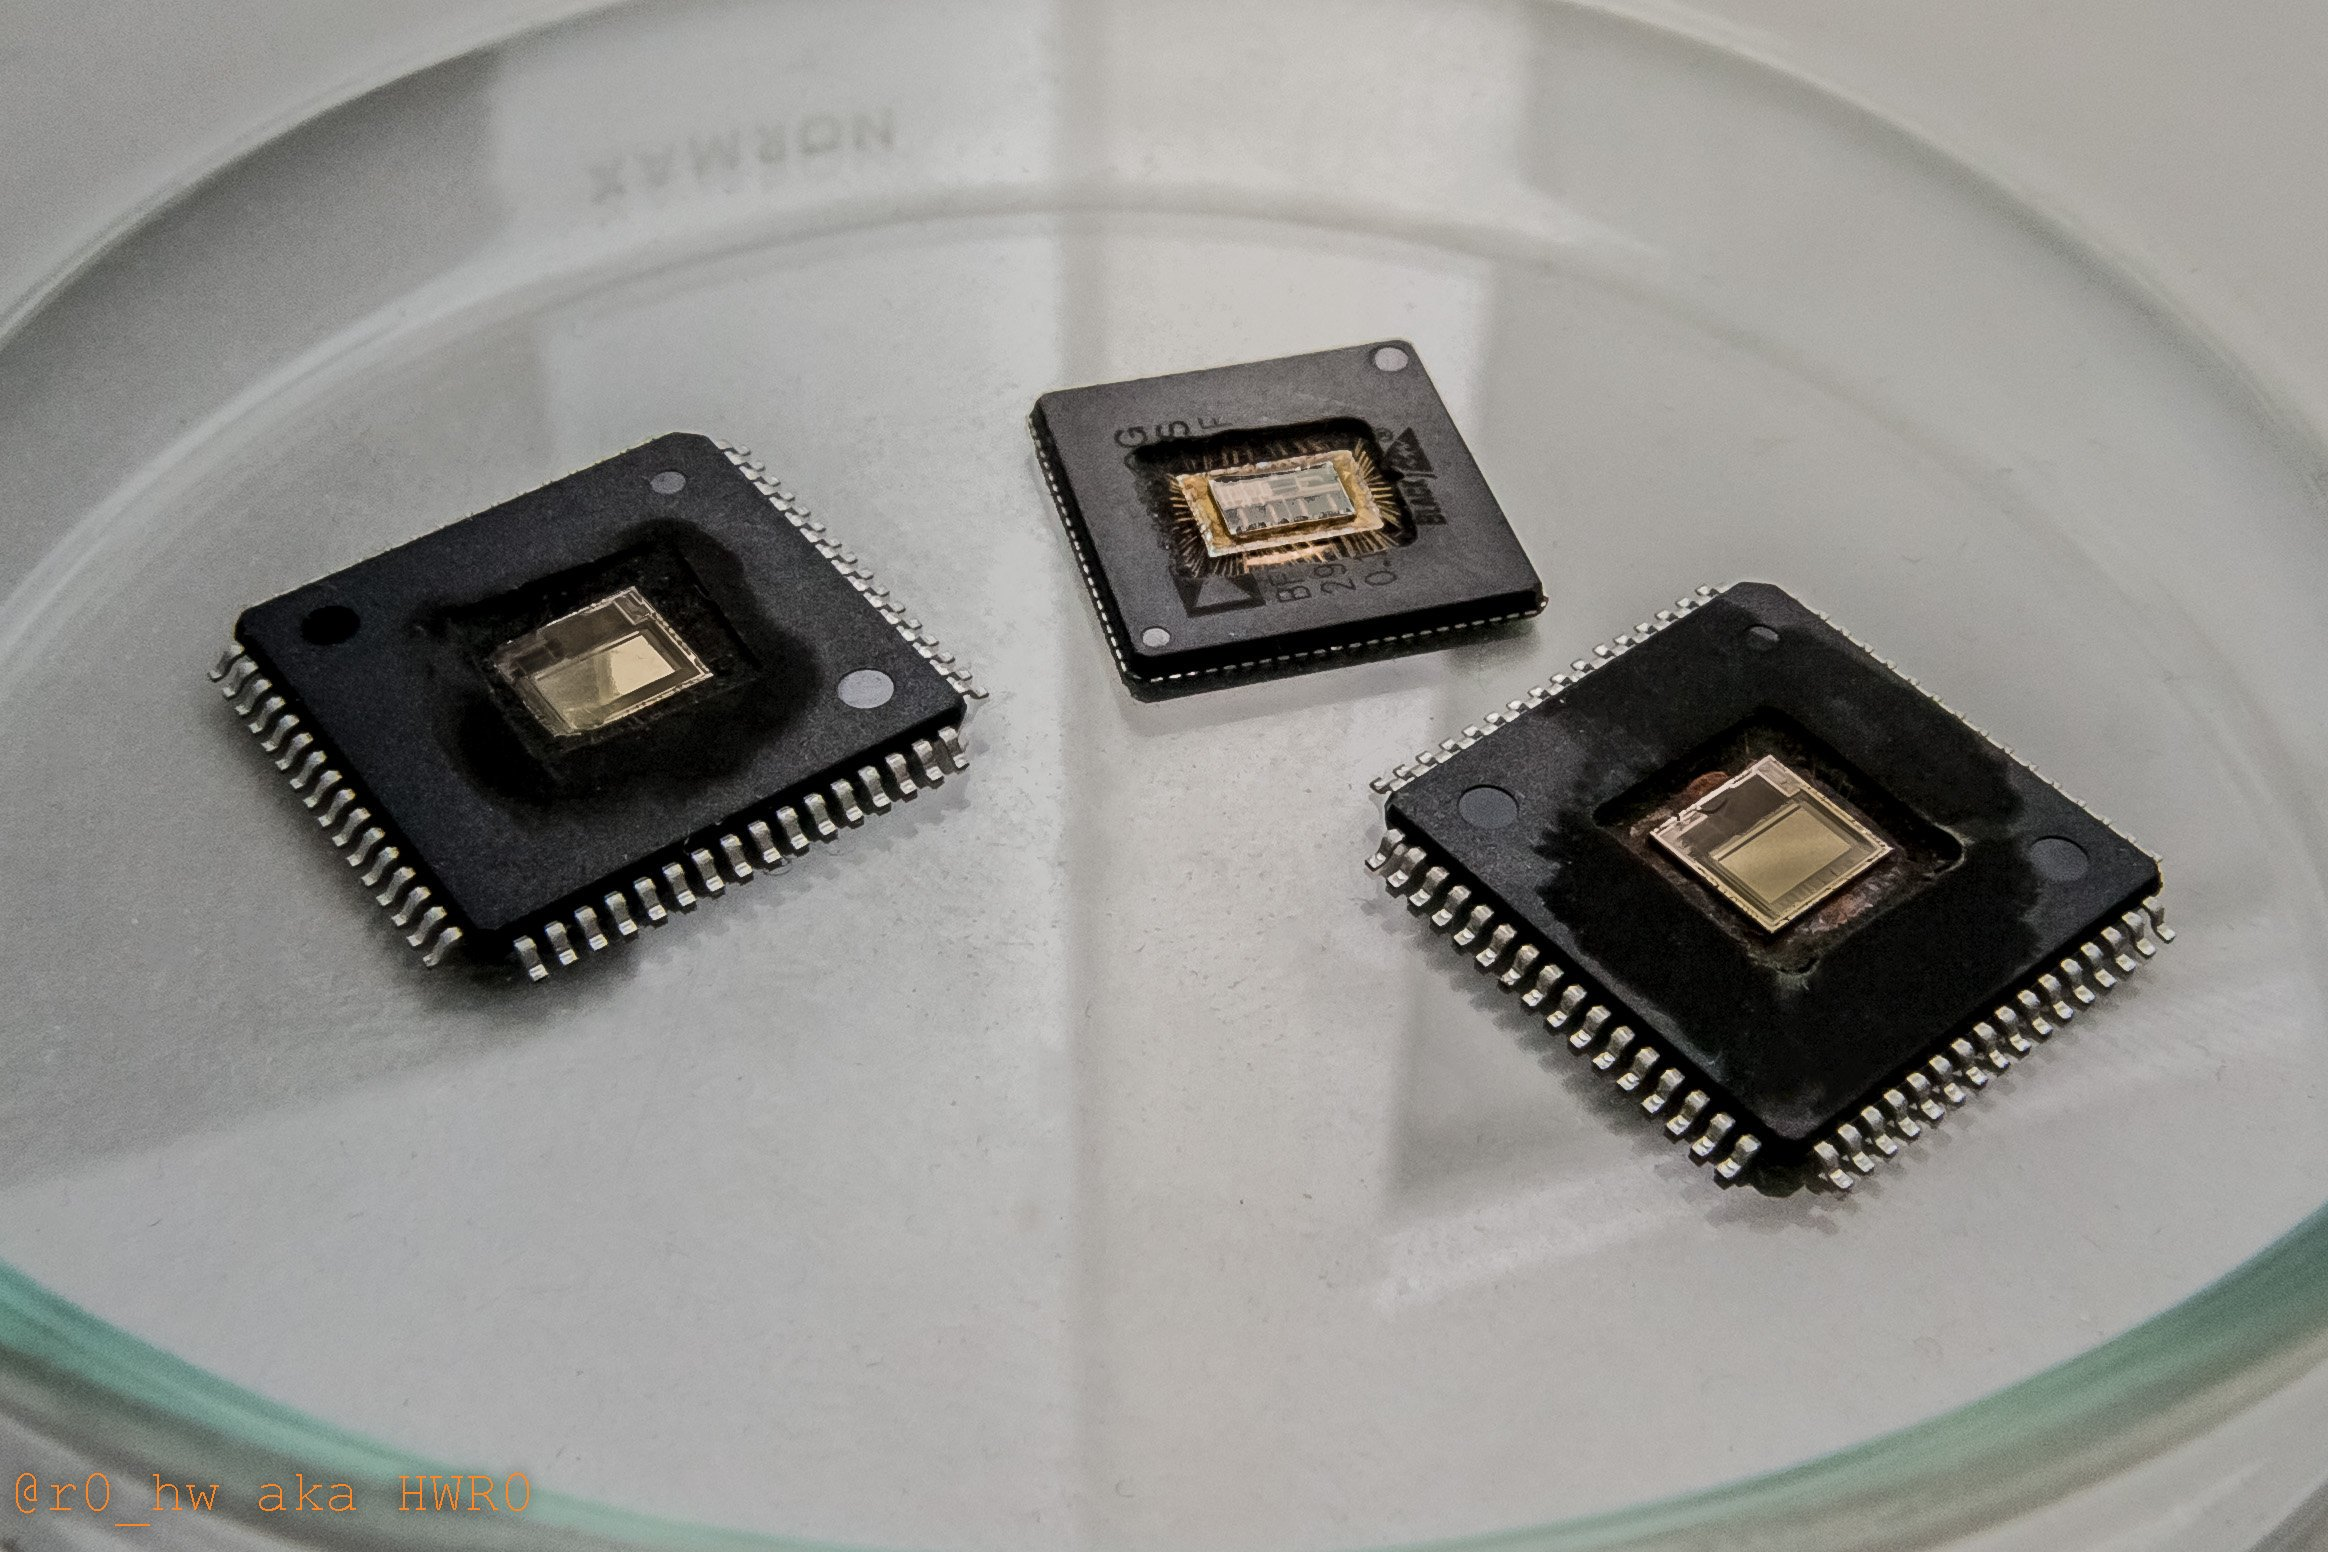
\includegraphics[width=.49\textwidth]{./decaping.jpg}%
                  \hfill
                  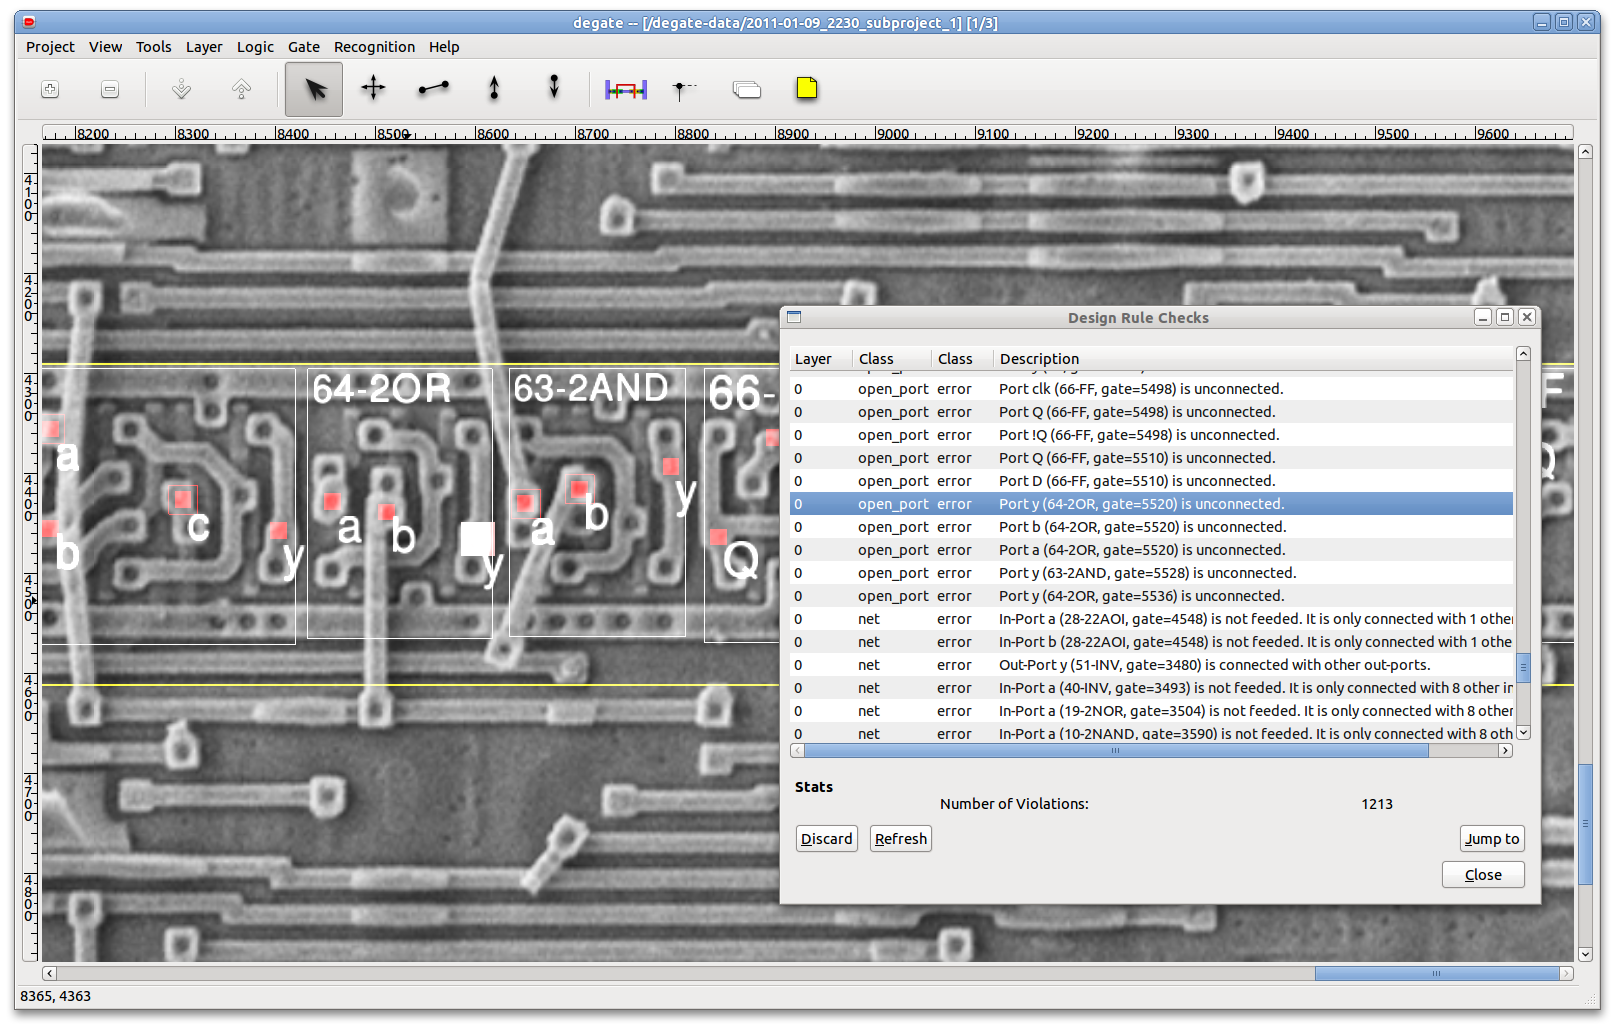
\includegraphics[width=.49\textwidth]{./degate.png}
                \end{figure}

\end{frame}

\begin{frame}
        \frametitle{Security Notions}

        \begin{itemize}
          \item {\bf Indistinguishability (IND) :} Ciphertexts should be
            indistinguishable from random strings,

          \item {\bf Non-Malleability (MD):} ``Given a ciphertext $C_1 = E(K, P 1)$,
it should be impossible to create another ciphertext, $C_2$ , whose corresponding
plaintext, $P_2$ , is related to $P_1$ in a meaningful way.''

        \end{itemize}

        \vspace{1 mm}

        Semantic Security (IND-CPA) is the most important security feature:
        \begin{itemize}
          \item Ciphertexts should be different when encryption is performed
            twice on the same plaintext,
          \item To achieve this, randomness is introduced into encryption /
            decryption: 

        \begin{itemize}
          \item $C = E(P, K, R)$
          \item $P = D(C, K, R)$
        \end{itemize}

        \end{itemize}
       \end{frame}


\begin{frame}
        \frametitle{Semantic Security}
        \begin{figure}
          \centering
          
\includegraphics[width=\textwidth]{d4-ecb.pdf}
        \end{figure}
        
\end{frame}


\begin{frame}
        \frametitle{Semantic Security}
For instance AES-ECB is not semantically secure - An attacker can build a
codebook to crack it.
        No Semantic Security without randomness

        \begin{itemize}
          \item
        \end{itemize}

\end{frame}

\begin{frame}
        \frametitle{Randomness}

        \begin{itemize}
          \item
        \end{itemize}

\end{frame}



\begin{frame}
        \frametitle{Generating Randomness}

        Random Number Generator:
        \begin{itemize}
          \item
        \end{itemize}

        Pseudo Random Number Generator:
        \begin{itemize}
          \item
        \end{itemize}

\end{frame}


\begin{frame}
        \frametitle{Entropy}

        \begin{itemize}
          \item
        \end{itemize}

\end{frame}

\begin{frame}
        \frametitle{Quantifying Security}
       RSA 2048 is roughly 100 bits security. 
        \begin{itemize}
          \item 
        \end{itemize}

\end{frame}



\begin{frame}
        \frametitle{Type of encryption}

        \begin{itemize}
          \item
        \end{itemize}

\end{frame}


\begin{frame}
        \frametitle{How thinks can go wrong}
        Some attacks requires less than CCA / CPA:
        \begin{itemize}
          \item Side Channel attacks as for instance Padding Oracle (Vaudenay Attacks)
        \end{itemize}

\end{frame}

\begin{frame}
  \begin{center}
    {\bf Encryption and Law Enforcement}
  \end{center}
\end{frame}

\begin{frame}
        \frametitle{2016 ENISA / EUROPOL joint statement}
        \begin{itemize}
          \item In the arms race between cryptographers and crypto-analysts. In
            terms of practical breaks, cryptographers are miles ahead.
          \item In a society that is ever more depending on the correct
            functioning of electronic communication services, technical
            protection of these service is mandatory,
          \item In the face of serious crimes, law enforcement may lawfully
            intrude privacy or break into security mechanisms of electronic communication,
          \item {\bf proportionality} - collateral damages (class breaks)
          \item Resolving the encryption dilemma: collect and share best
            practices to circumvent encryption.
        \end{itemize}
\end{frame}

\begin{frame}[allowframebreaks]
        \frametitle{Encryption Workarounds~\cite{kerr2017}}
        \begin{quote}
          Any effort to reveal an unencrypted version of a target's data that
          has been concealed by encryption.
        \end{quote}
        \begin{itemize}
          \item {\bf Try to get the key:}
          \begin{itemize}
        \item {\bf Find the key:} 
          \begin{itemize}
          \item physical searches for keys,
          \item password managers,
          \item web browser password database,
          \item in-memory copy of the key in computer's HDD / RAM.
          \item seize the key (keylogger).
          \end{itemize}
        \item {\bf Guess the key:},
          \begin{itemize}
            \item Whereas encryption keys are usually too hard to guess (eg.
              128bits security is $2^{128}$ trials (universe is $2^{88}$ ns old)),
            \item passphrases are usually shorter to be memorizable, and are
              linked to the key,
            \item some systems have limitations on sorts of passwords (eg. 4/6
              digits banking application),
            \item educated guess on the password from context,
            \item educated guess from owner's other passwords,
            \item dictionaries and password generation rules (\footnote{\url{https://hashcat.net/hashcat/}}).
            \item Offline / online attacks (eg. 13 digits pw: 25.000 on an
              iphone VS matter of minutes offline),
            \item + beware devices protection when online (eg. iphone erase on repeated failures).
          \end{itemize}
         
        \item {\bf Compel the key:}
          \begin{figure}
            \centering
            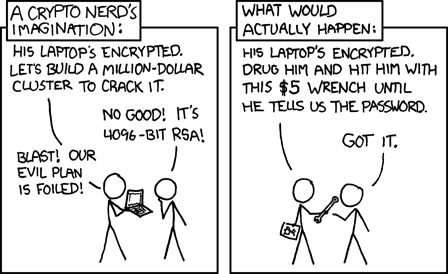
\includegraphics[width=180px]{security.png}
          \end{figure}
        \end{itemize}

          \item {\bf Try to access the PlainText without the key:}

        \begin{itemize}
          \item {\bf Exploit a Flaw:}

            \begin{itemize}
              \item Weakness in the algorithm (more on that later),
              \item weakness in the random-number generator (more on that later),
              \item weakness in the implementation,
              \item bugs (eg. Gordon's exploit on android in
                2015\footnote{\url{https://cve.circl.lu/cve/CVE-2015-3860}}),
              \item backdoors (eg. NSA NOBUS -Bullrun program- Dual EC-DRBG~\cite{eprint-2015-26238}
            \end{itemize}

          \item {\bf Access PlainText when in use:}

            \begin{itemize}
              \item Access live system memory,
              \item especially useful against Full Disk Encryption,
              \item Seize device while in use,
              \item remotely hack the device,
              \item ``Network Investigative Technique'' (eg. Playpen case
                against tor).
            \end{itemize}

\pagebreak 

          \item {\bf Locate a PlainText copy:}

            \begin{itemize}
              \item Avoid encryption entirely,
              \item cloud providers (eg. emails),
              \item remote cloud storage (eg. iCloud),
            \end{itemize}
 
        \end{itemize}

       \end{itemize}

      \vspace{5mm}

       {\bf Takeaways:}
       \begin{itemize}
        \item {\bf No workaround works every time:}  the fact that a target used
          encryption does not mean that the investigation is over.
        \item {\bf some workarounds are expensive:} exploiting.
        \item {\bf expertise may be have to be found outside of the
            governments:} vendors' assistance?
       \end{itemize}

 
        \framebreak

      Technically, we can retain that crypto-systems have weaknesses:

      \begin{itemize}
        \item key generation,
        \item key length,
        \item key distribution,
        \item key storage,
        \item how users enter keys into the crypto-system,
        \item weakness in the algorithm itself / implementation,
        \item system / computer running the algorithm,
        \item crypto system used in different points in time,
        \item {\bf users.}
      \end{itemize}

       
\end{frame}





\begin{frame}
  \begin{center}
    {\bf Cryptography and Network captures}
  \end{center}
\end{frame}

\begin{frame}
  \begin{center}
    {\bf D4 passiveSSL Collection}
  \end{center}
\end{frame}

\begin{frame}
  \begin{center}
    {\bf Leveraging OpenPGP metedata}
  \end{center}
\end{frame}

\begin{frame}
  \begin{center}
    {\bf Checking for weak crypto}
  \end{center}
\end{frame}

\begin{frame}
  \frametitle{Snake Oil Crypto\footnote{\url{https://github.com/d4-project/snake-oil-crypto}} - Problem Statement}
  IoT devices {\bf are often the weakest devices} on a network:
        \begin{itemize}
        \item Usually the result of cheap engineering,
        \item sloppy patching cycles,
        \item sometimes forgotten--not monitored,
        \item few hardening features enabled.
        \end{itemize}

        \vspace{10 mm} 

{\bf We feel a bit safer when they use TLS, but should we?}

\end{frame}

\begin{frame}
  \frametitle{Snake Oil Crypto - TLS Fingerprinting}
        {\bf Keep} a log of links between:
        \begin{itemize}
          \item x509 certificates,
          \item ports,
          \item IP address,
          \item client (ja3),
          \item server (ja3s),
        \end{itemize}
        \begin{quote}
        ``JA3 is a method for creating SSL/TLS client fingerprints that should be easy to produce on any platform and can be easily shared for threat intelligence.''\footnote{https://github.com/salesforce/ja3}
        \end{quote}

         {\bf Pivot} on additional data points during Incident Response 
\end{frame}

\begin{frame}
   \frametitle{Snake Oil Crypto -  Objectives}
   {\bf Collect} and {\bf store} x509 certificates and TLS sessions:
        \begin{itemize}
        \item Public keys type and size,
        \item moduli and public exponents,
        \item curves parameters.
        \end{itemize}
        {\bf Detect} anti patterns in crypto:
        \begin{itemize}
          \item Moduli that share one prime factor,
          \item Moduli that share both prime factors, or private exponents,
          \item Small factors,
          \item Nonces reuse / common preffix or suffix, etc. 
        \end{itemize}
        \vspace{5 mm}
        {\bf Focus on low hanging fruits that appeal to attackers}
\end{frame}


\begin{frame}[fragile]
   \frametitle{Snake Oil Crypto - RSA on IoT }
   Researchers have shown that several devices generated their keypairs
   at boot time without enough entropy\footnote{Bernstein, Heninger, and Lange: \url{http://facthacks.cr.yp.to/}}:
   
\begin{lstlisting}[frame=single, language=python]
prng.seed(seed)
p = prng.generate_random_prime()
// prng.add_entropy()
q = prng.generate_random_prime()
n = p*q
\end{lstlisting}

Given n=pq and n' = pq' it is trivial to recover the shared p by computing their
{\bf Greatest Common Divisor (GCD)}, and therefore {\bf both private keys}\footnote{\url{http://www.loyalty.org/~schoen/rsa/}}.

\end{frame}

\begin{frame}
   \frametitle{Snake Oil Crypto - GCD}
   In Snake-Oil-Crypto we compute GCD\footnote{using Bernstein's Batch GCD algorithm} between:
   
   \begin{itemize}
     \item between certificates having the same issuer,
     \item between certificates having the same subject,
     \item on keys collected from various sources (PassiveSSL, Certificate Transparency,
       shodan, censys, etc.),
   \end{itemize}

\vspace{10 mm}
  {\bf ``Check all the keys that we know of for vendor X''}

\end{frame}

\begin{frame}
   \frametitle{Snake Oil Crypto - MISP feed}
\begin{figure}
\centering
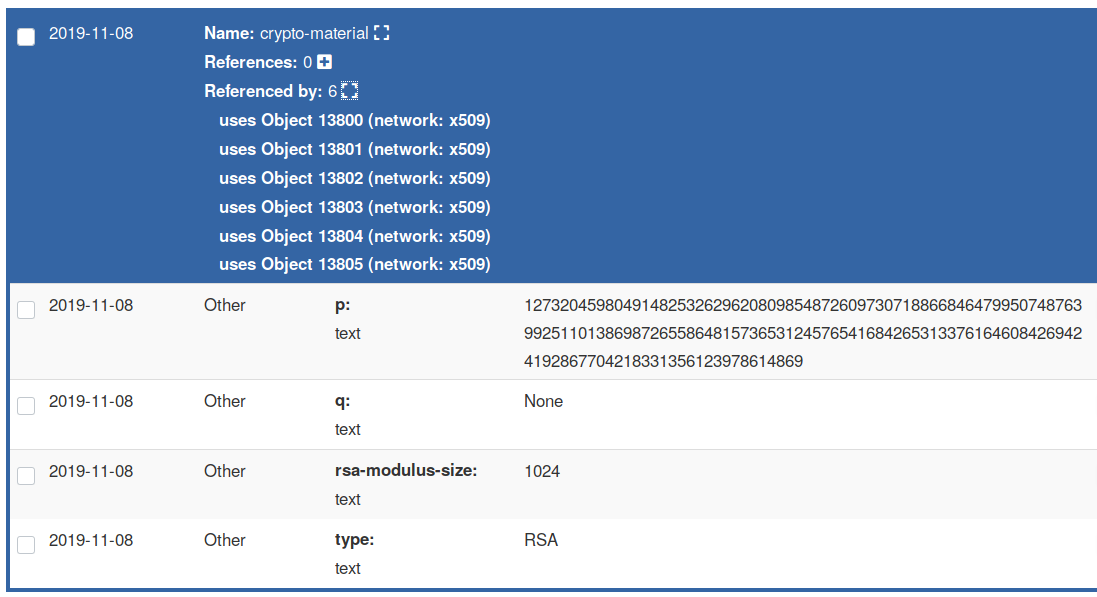
\includegraphics[width=\textwidth]{misp.png}
\end{figure}

\end{frame}

\begin{frame}
   \frametitle{Snake Oil Crypto - MISP feed}
   The MISP feed:
   \begin{itemize}
     \item {\bf Allows} for checking automatic checking by an IDS on hashed values,
     \item {\bf contains} thousands on broken keys from a dozen of vendors,
     \item {\bf will be accessible upon request (info@circl.lu).}
   \end{itemize}

   In the future:
    \begin{itemize}
     \item {\bf Automatic} the vendor checks by performing TF-IDF on x509's subjects, 
     \item {\bf automatic} vendors notification.
     \end{itemize}

\end{frame}


\begin{frame}
  \frametitle{First release}
  \begin{itemize}
  \item[\checkmark] sensor-d4-tls-fingerprinting
    \footnote{\url{github.com/D4-project/sensor-d4-tls-fingerprinting}}:
    {\bf Extracts} and {\bf fingerprints} certificates, and {\bf computes} TLSH fuzzy hash.
  \item[\checkmark] analyzer-d4-passivessl
    \footnote{\url{github.com/D4-project/analyzer-d4-passivessl}}:
    {\bf Stores} Certificates / PK details in a PostgreSQL DB.
  \item snake-oil-crypto 
    \footnote{\url{github.com/D4-project/snake-oil-crypto}}:
    {\bf Performs} crypto checks, push results in MISP for notification
  \item lookup-d4-passivessl
    \footnote{\url{github.com/D4-project/lookup-d4-passivessl}}:
    {\bf Exposes} the DB through a public REST API.
  \end{itemize}
\end{frame}



\begin{frame}
\frametitle{Get in touch if you want to join/support the project, host a passive ssl sensor or contribute}
\begin{itemize}
\item Collaboration can include research partnership, sharing of collected streams or improving the software.
\item Contact: info@circl.lu
\item \url{https://github.com/D4-Project} -  \url{https://twitter.com/d4_project}
\end{itemize}
\end{frame}

\nocite{*} 
\begin{frame}[allowframebreaks]
        \frametitle{References}
        \bibliographystyle{amsalpha}
        \bibliography{../references.bib}
\end{frame}

\end{document}
